\selectlanguage{english}
\clearpage
\section{Tool Evaluation and Framework Selection}

This chapter presents an evaluation of available tools and test frameworks that could be used to support the integration testing of IPC middleware. The goal is to identify solutions that align with the defined testing requirements and environmental constraints presented in the previous chapter. Based on a set of defined selection criteria, several tool candidates are reviewed and assessed in terms of their compatibility with eCAL and the specific demands of testing distributed communication systems.

\subsection{Selection Criteria}

To choose suitable testing tools and frameworks, several criteria were defined:

\begin{itemize}
	\item \textbf{Language Support:} The framework should support the languages already in use in the development environment, particularly C++ and Python.
	\item \textbf{Automation Capabilities:} Support for test automation, headless execution, and integration into CI/CD systems is essential.
	\item \textbf{Support for IPC Mechanisms:} Tools should be able to handle the orchestration of multi-process communication patterns, such as publish-subscribe and request-response.
	\item \textbf{Platform Compatibility:} The framework must work on Linux, as this is the primary target platform.
	\item \textbf{Observability and Reporting:} Tools should offer logging, result exporting, or structured test result visualization (e.g., HTML reports).
\end{itemize}

\subsection{Evaluation of Tool Candidates}

Figure~\ref{fig:mm_orchestration} presents an overview of evaluated tools and orchestration options in the form of a mind map.

\begin{figure}[H]
	\centering
	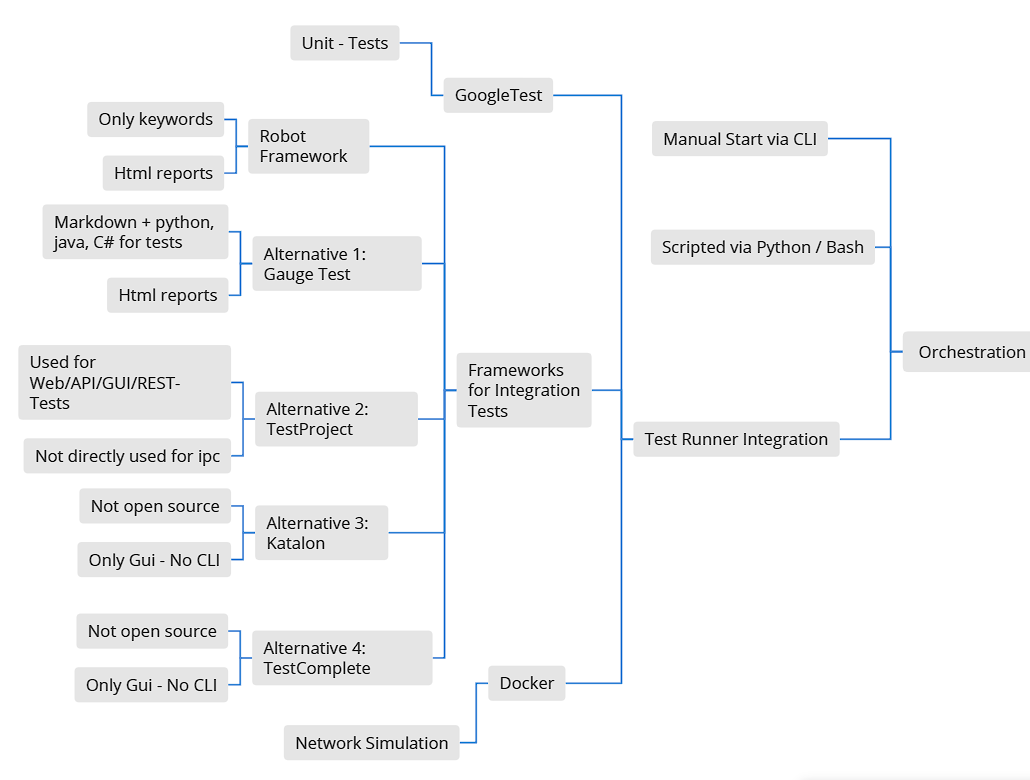
\includegraphics[width=\textwidth]{Images/mm_04_orchestration.png}
	\caption{Evaluation of orchestration and framework options for IPC testing}
	\label{fig:mm_orchestration}
\end{figure}

\subsubsection*{GoogleTest}

GoogleTest is a widely used testing framework for C++ applications. It provides many useful macros and assertions that help developers write automated tests for individual functions, classes, and modules. In the eCAL project, GoogleTest is already used to verify internal logic, data handling, and utility functions. This makes it a good choice for unit testing, especially during early development stages.
\\
\\
However, GoogleTest is mainly designed for unit testing and does not support tests that involve multiple running processes. Integration testing of IPC middleware usually requires testing communication between different processes such as publishers and subscribers. To use GoogleTest in this context, additional scripts or wrapper functions are needed to start processes and simulate communication. While this is possible, it increases the complexity of test setups and reduces maintainability. Therefore, GoogleTest should be combined with other tools when performing full integration tests. More information is available in the official GoogleTest documentation~\cite{GoogleTestDocs}.

\subsubsection*{Robot Framework}

Robot Framework is a general-purpose, open-source test automation framework. It follows a keyword-driven approach, allowing users to write tests in a readable and structured way. Tests are usually written in plain text and can be run through the command line or integrated into automated systems.
\\
\\
One of the key strengths of Robot Framework is its flexibility and support for integration testing. With built-in libraries such as \texttt{Process}, \texttt{OperatingSystem}, and \texttt{BuiltIn}, it can start and stop applications, check logs, and validate output. These features are especially helpful for testing IPC middleware like eCAL, where several processes must run in parallel and communicate correctly. For example, Robot Framework can launch both publishers and subscribers, wait for data exchange, and verify the results.
\\
\\
Another important feature is automatic report generation. After each test run, Robot Framework produces HTML and XML reports that show test results, timing, and logs. This is very useful for continuous integration pipelines that run tests regularly. The official Robot Framework User Guide provides further details~\cite{RobotFrameworkDocs}.

\subsubsection*{Gauge Test}

Gauge is a modern test framework developed by ThoughtWorks. It lets users write test scenarios in Markdown format, which helps make tests easier to read and maintain. These scenarios are then connected to test code written in programming languages like Java, Python, or C\#. Gauge also supports running tests in parallel and generating HTML reports.
\\
\\
Although Gauge has many useful features, it is mostly used for testing web applications, APIs, and user interfaces. It is not specifically designed for backend systems like IPC middleware. Also, its community is relatively small, and there are fewer plugins available compared to larger frameworks.
\\
\\
Using Gauge for testing IPC would require custom scripts and additional effort to manage process orchestration. Because of this, Gauge is not the best fit for testing systems like eCAL. Further documentation can be found on the official Gauge website~\cite{GaugeDocs}.

\subsubsection*{TestProject, Katalon, and TestComplete}

TestProject, Katalon, and TestComplete are test tools mainly used for testing web interfaces, APIs, and desktop applications. They often include graphical interfaces for designing and running tests, and they support features like recording user actions and parameterizing input values.
\\
\\
However, these tools are not intended for testing IPC systems. They do not support low-level message handling or process orchestration, which are important when testing middleware like eCAL. In addition, most of these tools are not open source, and they often rely on graphical interfaces, which makes them less suitable for headless environments or automation using Docker and CLI.
\\
\\
For these reasons, these tools are not recommended for integration testing of eCAL or similar IPC frameworks. More information can be found in their official documentation~\cite{TestProjectDocs,KatalonDocs,TestCompleteDocs}.



\subsection{Feasibility for eCAL Integration}

Following the evaluation of several testing frameworks, Robot Framework was identified as the most appropriate tool for conducting integration testing of systems based on the eCAL middleware. It meets the key technical requirements, including support for keyword-driven scripting, automation of command-line processes, and the orchestration of multiple running applications. These capabilities are essential for testing publish-subscribe communication patterns and service-based interactions, which are common in IPC middleware systems.
\\
\\
While Robot Framework is suited for system-level and integration testing, GoogleTest will remain the preferred tool for unit testing within the eCAL source code. Its strong support for C++ and its existing integration into the eCAL development workflow make it a practical choice for verifying individual modules, internal logic, and data structures at a low level. By using Robot Framework for high-level process orchestration and GoogleTest for component-level validation, a complete and balanced testing strategy can be established for the entire middleware system.

